\section{Background}\label{section2}

% This section provides a brief overview of the basic concepts related to: (i) SPL and variabilities; (ii) the SMarty approach, for variability management; and (iii) mobile learning.

\subsection{Software Product Lines}

A Software Product Line (SPL) enables the creation of software-intensive systems that share and manage a set of features for satisfying the specific needs of a particular domain. Commonalities are shared by all derived products, while variabilities represent the scope of customization supported by them \cite{bockle05,vanderlinden07}.

The concept of SPL is suitable for domains in which products that share common features and a well-defined set of variabilities are demanded. At its essence, the conception of an SPL involves domain engineering and product development, both under technical and organizational management perspectives \cite{bockle05,vanderlinden07}.

The variabilities can be initially identified and represented by means of features, relevant and visible characteristics to stakeholders of a particular domain \cite{bosch01}. The precise and explicit representation and management of variabilities enable a consistent generation of specific products in an SPL \cite{chen11,galster2014}. 

\subsection{SMarty: an Approach for Variability Management}

The proper management of variabilities has great relevance to ensure that all the benefits of SPL are obtained. Therefore, different approaches related to the variability management have been proposed by the research community, such as SMarty.  \cite{chen11,capilla13}.  

According to OliveiraJr et al \cite{oliveirajr10}, SMarty is a variability management approach composed of a UML (Unified Modeling Language) 2.4 profile (SMartyProfile) and supported by a systematic process (SMartyProcess), related to the main SPL activities. SMartyProcess defines a set of guidelines that supports the application of stereotypes and tagged-values. The guidelines ensure the identification and representation of variabilities and enabled the evolution of SPL, whereas the process incrementally and iteratively guarantees the identification of new variabilities and evolution of the SPL core assets.

% Another benefit from the use of SMarty is visibility regarding the relationship among the feature model and variabilities in the UML diagrams. The variabilities composed of variation points are fully represented. Therefore, there are no additional documents for the development of SPL \cite{oliveirajr10}.

The UML diagrams supported by SMarty (use case, class, sequence, component and activity) represent the static and dynamic aspects of software products. The SMarty effectiveness in identifying and representing variabilities in the UML models has been experimentally evaluated \cite{marcolino13,marcolino14a,marcolino14b,bera15}. The results provided initial evidence of the SMarty effectiveness. In addition, they lead to the empirically evolution of SMarty in general.

\subsection{M-SPLear\allowbreak ning: an SPL for M-learning Applications}

% The rapid growth of information and communication technologies has favored the emergence of new methods for teaching and learning and innovative ways for facing the shortcomings of traditional education \cite{west12}.

M-learning is characterized by its ability to provide a strong interaction between learners and instructors, who not only access a virtual learning environment, but also contribute to and actively participate in the knowledge construction process through mobile devices anytime and anywhere \cite{kukulska05}. 

% The interaction through mobile devices provides other benefits than accessibility, convenience and communication. In this sense, mobile devices have technologies and sensors that can be used in support of educational activities: (i) accelerometer; (ii) GPS (Global Positioning System); (iii) camera; (iv) touch screen; and (v) fingerprint \cite{lane10}. This allows m-learning applications to explore such resources, engaging learners and stimulating their interaction with teachers \cite{picek13,fazlina13}.

However, m-learning is still considered an incipient concept, as it has limitations that hamper its effective development and adoption. For instance, even with the increasing demand for m-learning applications, few studies have addressed development issues through a strategy of systematic reuse, such as SPL, in the mobile learning domain.  

Based on the concepts and ideas summarized in this section, we have worked on the establishment of an SPL for the m-learning domain, named M-SPLear\allowbreak ning \cite{falvojr14,falvojr14b}. Its conception utilized the proactive approach proposed by \cite{krueger02}, which includes the following phases: (i) Domain Engineering; (ii) Architecture; and (iii) Design.

The proactive approach is appropriate when the requirements for the set of products to be created are stable and can be defined in advance. Therefore, M-SPLear\allowbreak ning derived a catalog of requirements proposed by \cite{filho13}. In addition, to standardize the variability management, the SMarty was used in all the diagrams modeled for the SPL.

In this sense, the most representative asset considering M-SPLear\allowbreak ning's variability management is the SMarty-based Component Diagram (Figure \ref{fig:msplearning-design}). This diagram is the main artifact of the Design phase, because it presents the variabilities, commonalities and interactions between the features supported by the SPL. Therefore, we have an overview of the product line and its domain modeling.

\begin{figure*}[!ht]
\centering
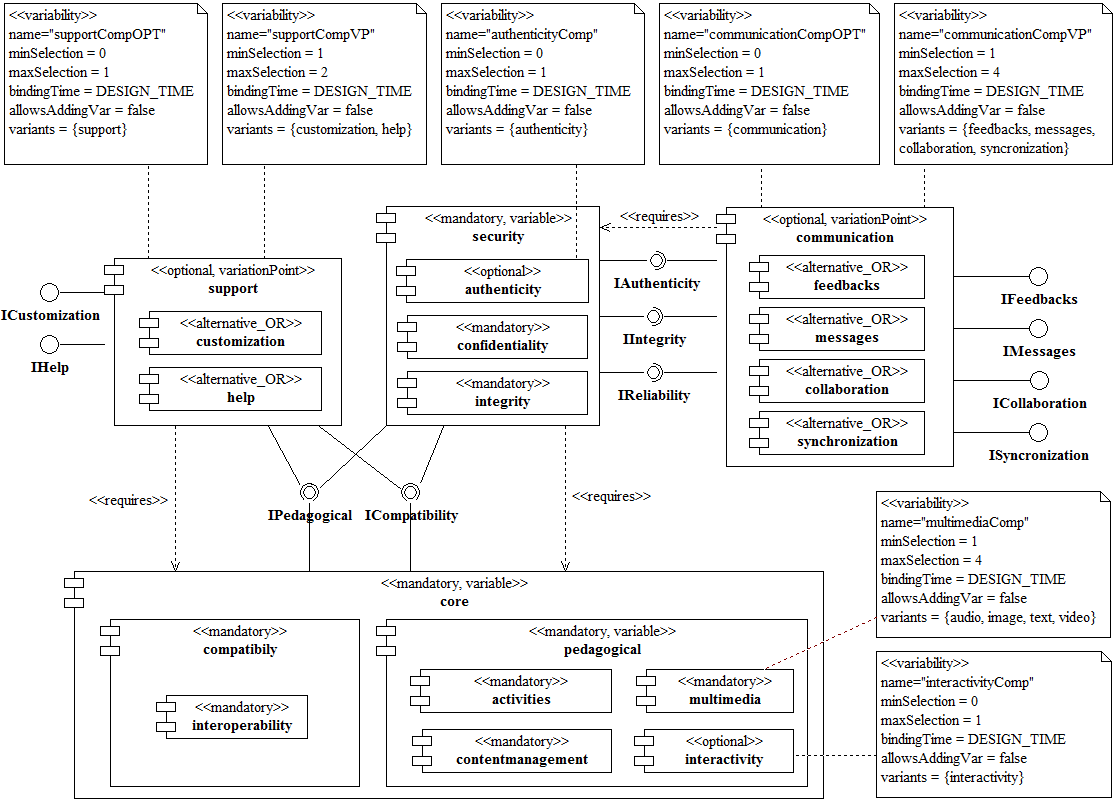
\includegraphics[width=1.05\textwidth]{MSPLDesign.png}
\centering
\caption{M-SPLearning: SMarty-based Components Diagram.}
\label{fig:msplearning-design}
\end{figure*}

Finally, with the support of these approaches and tools it was possible to instantiate our SPL, allowing an experimental evaluation of the products generated by M-SPLearning. The following section details our experiment and its results.
